%%%%%%%%%%%%%%%%%%%%%%%%%%%%%%%%%%%%%%%%%%%%%%%%%%%
%
%  New template code for TAMU Theses and Dissertations starting Fall 2016.  
%
%
%  Author: Sean Zachary Roberson
%  Version 3.17.09
%  Last Updated: 9/21/2017
%
%%%%%%%%%%%%%%%%%%%%%%%%%%%%%%%%%%%%%%%%%%%%%%%%%%%

%%%%%%%%%%%%%%%%%%%%%%%%%%%%%%%%%%%%%%%%%%%%%%%%%%%%%%%%%%%%%%%%%%%%%%%
%%%                           SECTION II
%%%%%%%%%%%%%%%%%%%%%%%%%%%%%%%%%%%%%%%%%%%%%%%%%%%%%%%%%%%%%%%%%%%%%%


\chapter{PARALLEL TRANSPORT SWEEPS}
As mentioned in the previous chapter, a transport sweep is set up by overlaying a domain with a finite element mesh and solving the transport equation cell by cell using a discontinuous finite element approach. A task-dependence graph gives the order in which cells are solved, as shown in Fig. \ref{tdg}. A transport sweep can be solved in parallel in order to obtain the solution faster, as well as distribute the problem across many processors for memory intensive problems. 

In PDT, a transport sweep can be performed on a structured Cartesian or arbitrary polyhedral mesh. Sweeping on an unstructured mesh presents two challenges: maintaining sweep efficiency on a massively parallel scale and keeping non-concave sub-domains to avoid cycles. PDT has already proven the ability to perform massively parallel transport sweeps on structured meshes. As part of previous efforts in PDT, researchers have outlined three important properties for parallel sweeps. 

A parallel sweep algorithm is defined by three properties \cite{mpadams2013} :
\begin{itemize}
\item partitioning: dividing the domain among available processors,
\item aggregation: grouping cells, directions, and energy groups into tasks,
\item scheduling: choosing which task to execute if more than one is available.
\end{itemize}

The basic concepts of parallel transport sweeps, partitioning, aggregation, and scheduling, are most easily described in the context of a  transport sweep that takes place on a structured Cartesian mesh. Furthermore, the work detailed in Chapters \ref{cha:lb} and \ref{cha:tts} utilize aspects of the structured transport sweep.

In a regular grid, we have the  number of cells in each Cartesian direction: $N_x, N_y, N_z$. These cells are aggregated into ``cellsets'', using aggregation factors $A_x, A_y, A_z$. If $M$ is the number of angular directions per octant, $G$ is the total number of energy groups, and $N$ is the total number of cells, then the total fine-grain work units is $8MGN$. The factor of 8 is present as $M$ directions are swept for all 8 octants. The finest-grain work unit is the calculation of a single direction and energy group's unknowns in a single cell, or $\psi_{m,g}$ for a single cell.

Fine-grain work units are aggregated into coarser-grained units called \textit{tasks}. A few terms are defined that describe how each variable is aggregated.
\begin{itemize}
\item $A_x = \frac{N_x}{P_x}$, where $N_x$ is the number of cells in $x$ and $P_x$ is the number of processors in $x$.
\item $A_y = \frac{N_y}{P_y}$, where $N_y$ is the number of cells in $y$ and $P_y$ is the number of processors in $y$.
\item $A_z$ = a selectable number of z-planes of $A_x A_y$ cells.
\item $N_g = \frac{G}{A_g}$
\item $N_m = \frac{M}{A_m}$
\item $N_k = \frac{N_z}{P_z A_z}$
\item $N_k A_x A_y A_z = \frac{N_x N_y N_z}{P_x P_y P_z}$
\end{itemize}

It follows that each process owns $N_k$ cellsets (each of which is $A_z$ planes of $A_x A_y$ cells), $8N_m$ angle-sets, and $N_g$ group-sets for a total of $8N_m N_g N_k$ tasks.

One task contains $A_x A_y A_z$ cells, $A_m$ directions, and $A_g$ groups. Equivalently, a task is the computation of one cellset, one groupset, and one angleset, with the completion of one task defined as a stage.  The stage is particularly important when assessing sweeps against analytical performance models. 

Equation ~\eqref{paralleleff} approximately defines parallel sweep efficiency:
\begin{equation}\label{paralleleff}
\begin{split}
\epsilon &\approx \frac{T_{\text{task}} N_{\text{tasks}}}{[N_{\text{stages}}] [T_{\text{task}} + T_{\text{comm}}]} \\
            &\approx\frac{1}{[1+\frac{N_{\text{idle}}}{N_{\text{tasks}}}][1 + \frac{T_{\text{comm}}}{T_{\text{task}}}]},
\end{split}
\end{equation}
where $N_\text{idle}$ is the number of idle stages per processor, $N_\text{tasks}$ is the number of tasks each processor performs, $T_\text{comm}$ is the time to communicate after completion of a task, and $T_\text{task}$ is the time it takes to compute one task.
Equations ~\eqref{Tcomm} and ~\eqref{Ttask} show how $T_{\text{comm}}$ and $T_{\text{task}}$ are calculated:
\begin{equation}
T_{\text{comm}} = M_L T_{\text{latency}} + T_{\text{byte}} N_{\text{bytes}}
\label{Tcomm}
\end{equation}
\begin{equation}
T_{\text{task}} = A_x A_y A_z A_m A_g T_{\text{grind}},
\label{Ttask}
\end{equation}
where $T_{\text{latency}}$ is the message latency time, $T_{\text{byte}}$ is the time required to send one byte of message, $N_{\text{bytes}}$ is the total number of bytes of information that a processor must communicate to its downstream neighbors at each stage, and $T_{\text{grind}}$ is the time it takes to compute a single cell, direction, and energy group. $M_L$ is a latency parameter that is used to explore performance as a function of increased or decreased latency. Note that Eq. \ref{Ttask} is idealized as it does not take into account overhead in various parts of the sweep implementation.

Before expanding on the proposed method of partitioning and scheduling for parallel transport sweeps, a quick review of some transport sweep algorithms is necessary. Our method will expand on PDT's sweep algorithm\cite{mpadams2013}, which is an extension of the popular KBA algorithm\cite{KBA}.

\section{The KBA Algorithm}

Several parallel transport sweep codes use KBA partitioning in their sweeping, such as Denovo \cite{denovo} and PARTISN \cite{partisn}. The KBA partitioning scheme and algorithm was developed by Koch, Baker, and Alcouffe \cite{KBA}.

The KBA algorithm traditionally chooses $P_z = 1, A_m = 1, G = A_g = 1, A_x = N_x/P_x, A_y = N_y/P_y$, with $A_z$ being the selectable number of z-planes to be aggregated into each task. This partitions the domain into longer, thin columns. With $N_k = N_z/A_z$, each processor performs $N_{\text{tasks}} = 8MN_k$ tasks. KBA uses a ``pipelining" or assembly line approach where new work is started before old work is fully completed. Figure \ref{pipeline_example} shows an example of pipelining the angular work of a quadrant.

\begin{figure}[H]
\centering
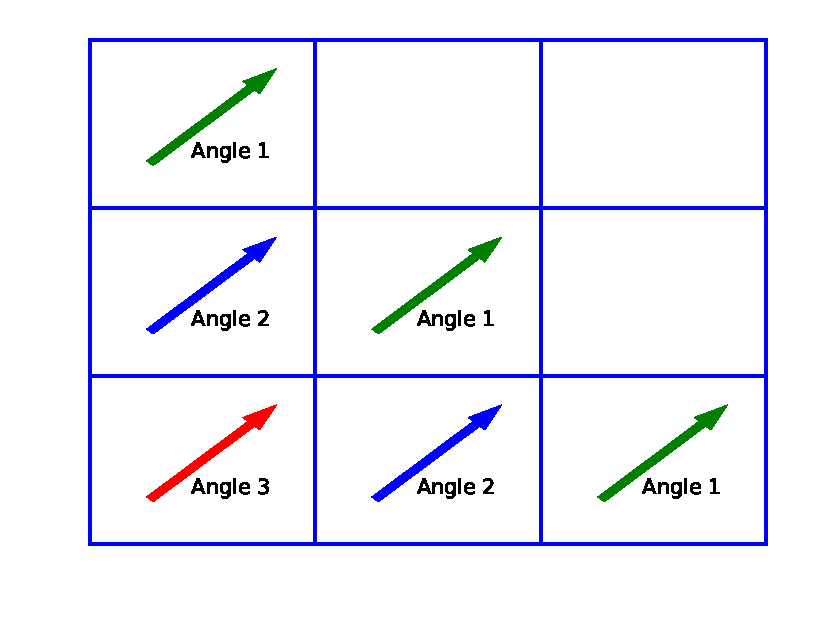
\includegraphics[scale=0.75,trim={0cm 1cm 0cm 0cm},clip]{../figures/pipeline_example.pdf}
\caption{An example showing the pipelining of angular work from the lower left quadrant.}
\label{pipeline_example}
\end{figure}

In Fig. \ref{pipeline_example}, we see that as soon as a processor is free to solve the next angle with the same sweep ordering, it begins immediately. KBA introduced pipelining in order to combat the inherent inefficiencies of waiting for all processors to complete a sweep in a direction before starting the next angle. 

There are two variants to the KBA algorithm, ``successive in angle, successive in quadrant", and ``simultaneous in angle, successive in quadrant".  With ``successive in angle, successive in quadrant", an octant pipelines its angular work, and once all directions are complete the opposing octant pipelines them back. This is then done for the remaining octant pairs. With ``simultaneous in angle, successive in quadrant", all angles from one octant are simultaneously solved, and upon completion the opposing octant solves them. This is then done for the remaining octant pairs. The KBA parallel efficiency\cite{mpadams2013} for ``successive in angle, successive in quadrant" is:
\begin{equation}
  \epsilon_{KBA} \approx \frac{1}{[1 + \frac{4(P_x+P_y-2)}{8MN_k}][1 + \frac{T_{\text{comm}}}{T_{\text{{task}}}}]}.
\end{equation}

\section{PDT's extension of KBA}\label {pdt_extension}

PDT's extension of KBA does not limit $P_z, A_m, G,$ or $A_g$. In addition, all 8 octants (4 quadrants in 2D) begin work immediately. Unlike KBA, PDT's scheduling requires conflict resolution in its algorithm, as the pipelines from all octants will end up intersecting toward the middle of the processor domain.

If two or more tasks reach a processor at the same time, PDT employs a tie breaking strategy:

\begin{enumerate}
	\item The task with the greater depth-of-graph remaining (simply, more work remaining) goes first.
	\item If the depth-of-graph remaining is tied, the task with $\Omega_x > 0$ wins.
	\item If multiple tasks have $\Omega_x > 0$, then the task with $\Omega_y > 0$ wins.
	\item If multiple tasks have $\Omega_y > 0$, then the task with $\Omega_z > 0$ wins.
\end{enumerate}

Given these conflict resolution techniques, the minimum possible number of stages for given partitioning parameters $P_i$ and $A_j$ is $2N_{\text{fill}} + N_{\text{tasks}}$. $N_{\text{fill}}$ is both the minimum number of stages before a sweepfront can reach the center-most processors and the number needed to finish a direction's sweep after the center-most processors have finished. Equations \ref{nfill}, \ref{nidle}, and \ref{ntasks} define $N_{\text{fill}}, N_{\text{idle}}$, and $N_{\text{tasks}}$:

\begin{equation}
N_\text{fill} = \frac{P_x}{2} - 1 + \frac{P_y}{2} - 1 + N_k (\frac{P_z}{2} - 1)
\label{nfill}
\end{equation}
\begin{equation}
N_\text{idle} = 2N_{\text{fill}}
\label{nidle}
\end{equation}
\begin{equation}
N_\text{tasks} = 8N_mN_gN_k
\label{ntasks}
\end{equation}

Plugging these definitions into Eq. \ref{paralleleff}, the PDT optimal parallel efficiency\cite{mpadams2013} is:
\begin{equation}
	\epsilon \approx \frac{1}{ [1 + \frac{P_x + P_y - 4 + N_k(P_z -2)}{8MGN_k/(A_m A_G)} ]  [ 1 +  \frac{T_{\text{comm}}}{T_{\text{task}}} ]}
\end{equation}
